\section{Configuração dos Experimentos}

Este capítulo apresenta os resultados obtidos nas implementações avaliadas neste
trabalho. A análise considera três aspectos principais: o tempo de geração do
grafo R-MAT, o desempenho do Kernel 2 do Graph500, correspondente à busca em
largura, e o desempenho da biblioteca de travessia de grafos executada
majoritariamente em GPU.

A métrica principal usada para a BFS é TEPS (\textit{Traversed Edges Per
Second}), apresentada na Seção~\ref{sec:graph500-metricas}. Para facilitar a
leitura das tabelas, os resultados de BFS são apresentados em GTEPS, isto é,
bilhões de arestas percorridas por segundo. O valor usado para comparação é a
mediana de TEPS das buscas realizadas, pois o Graph500 executa múltiplas BFS a
partir de raízes distintas.

Foram considerados dois ambientes experimentais. O primeiro foi o computador
pessoal utilizado durante o desenvolvimento, com processador Ryzen 5 5600X, 32 GB
de memória RAM e uma GPU NVIDIA RTX 5060 Ti com 16 GB de memória. O segundo foi
um ambiente GB200 com processador Grace, 128 threads de CPU e quatro GPUs GB200.
Em todos os experimentos reportados, o fator de arestas foi igual a 16.

\section{Implementações Comparadas}

Foram consideradas três implementações durante a avaliação.

\begin{itemize}
\item \textbf{Graph500 MPI em CPU}: implementação de referência do Graph500,
executada em CPU com processos MPI. No computador pessoal foram usados 12
processos; no GB200 foram usados 128 threads/processos de execução na referência.
\item \textbf{Graph500 CUDA/NVSHMEM híbrido}: implementação em GPU em que a
expansão da fronteira é feita por CUDA e as atualizações remotas são feitas com
NVSHMEM, mas a CPU ainda coordena a passagem entre níveis da BFS. No computador
pessoal essa versão foi executada com uma GPU.
\item \textbf{Biblioteca GPU}: versão refatorada em que a geração do grafo, a
conversão da representação e a BFS são organizadas como componentes de uma
biblioteca. Nessa versão, o laço principal da BFS é mantido na GPU. No computador
pessoal foi usada uma GPU; no GB200 foram usadas quatro GPUs.
\end{itemize}

Essa separação permite avaliar duas questões. A primeira é comparar a
implementação Graph500 em GPU com a referência em CPU. A segunda é avaliar se a
refatoração em biblioteca melhora o desempenho ao mover mais controle da BFS para
o dispositivo.

\section{Graph500 no Computador Pessoal}

O primeiro conjunto de resultados compara a implementação de referência em CPU
com a implementação CUDA/NVSHMEM híbrida no computador pessoal. As execuções
foram realizadas de \texttt{SCALE=12} até \texttt{SCALE=22}, com fator de arestas
igual a 16. As execuções desse conjunto foram realizadas sem validação, para
isolar o tempo do Kernel 2.

A Tabela~\ref{tab:pc-graph500-teps} mostra a mediana de GTEPS para cada escala.

\begin{table}[H]
\centering
\resizebox{\textwidth}{!}{
\begin{tabular}{c|c|c|c}
\hline
SCALE & CPU referência (GTEPS) & CUDA/NVSHMEM híbrido (GTEPS) & Melhor implementação \\
\hline
12 & 0,118836 & 0,013309 & CPU \\
13 & 0,161919 & 0,020870 & CPU \\
14 & 0,184855 & 0,031873 & CPU \\
15 & 0,187101 & 0,040772 & CPU \\
16 & 0,207790 & 0,061139 & CPU \\
17 & 0,219391 & 0,085607 & CPU \\
18 & 0,226187 & 0,110411 & CPU \\
19 & 0,226301 & 0,143063 & CPU \\
20 & 0,208037 & 0,185881 & CPU \\
21 & 0,210570 & 0,236604 & GPU \\
22 & 0,195437 & 0,253907 & GPU \\
\hline
\end{tabular}
}
\caption{Mediana de GTEPS no computador pessoal para a referência em CPU e a versão CUDA/NVSHMEM híbrida.}
\label{tab:pc-graph500-teps}
\end{table}

Os resultados mostram que a implementação em CPU é superior nas escalas pequenas
e médias. Isso ocorre porque, nessas escalas, o custo fixo de inicialização,
sincronização e coordenação da execução em GPU ainda é alto em relação ao volume
de arestas percorridas. A partir de \texttt{SCALE=21}, a versão CUDA/NVSHMEM
híbrida passa a superar a referência em CPU. Em \texttt{SCALE=22}, a versão GPU
atinge 0,253907 GTEPS, contra 0,195437 GTEPS da referência, um ganho de
aproximadamente $1{,}30$ vez.

A Figura~\ref{fig:pc-graph500-teps} apresenta a mesma tendência de forma visual.

\begin{figure}[H]
\centering
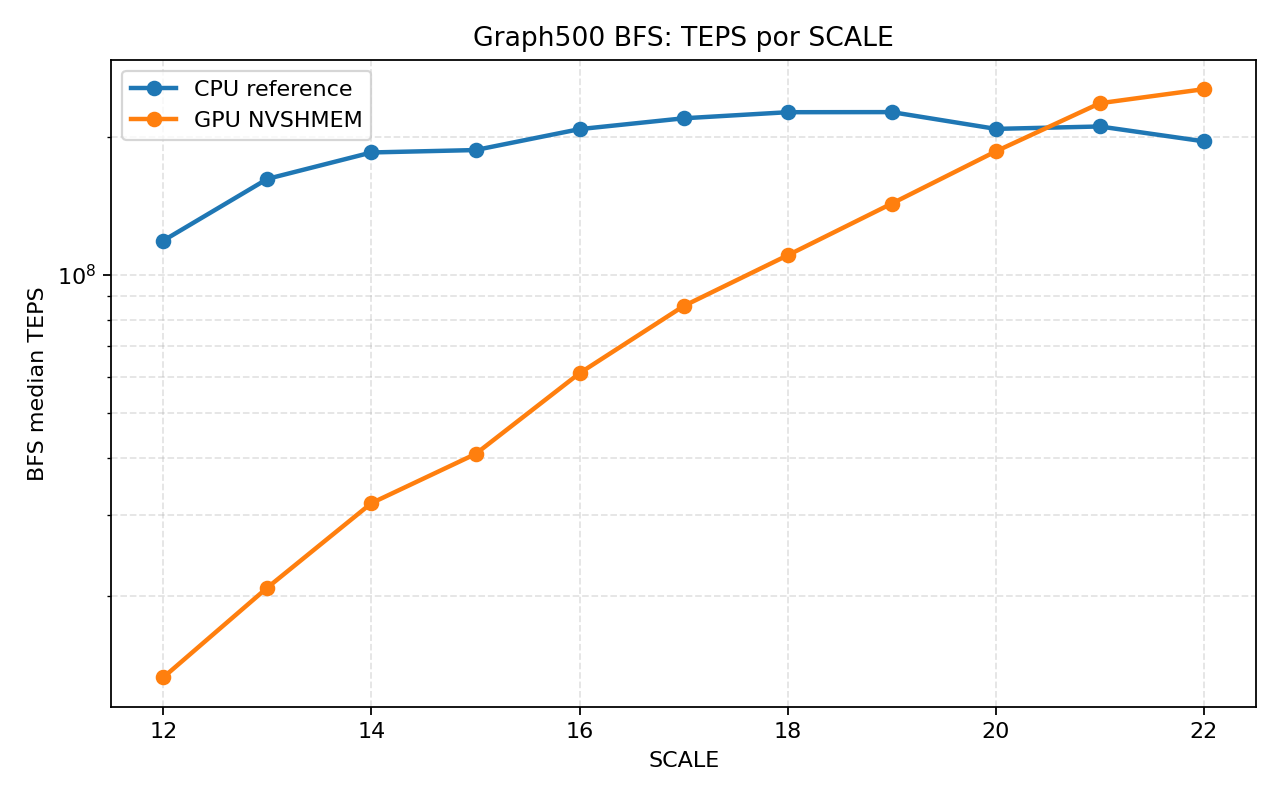
\includegraphics[width=0.9\textwidth]{resultados/resultado_computador_pessoal_graph500_nvshmem/teps_by_scale.png}
\caption{Mediana de GTEPS por escala no computador pessoal.}
\label{fig:pc-graph500-teps}
\end{figure}

\section{Geração do Grafo no Computador Pessoal}

Além do Kernel 2, também foi medido o tempo de geração R-MAT. A
Tabela~\ref{tab:pc-graph500-geracao} resume esses tempos para algumas escalas
representativas.

\begin{table}[H]
\centering
\resizebox{\textwidth}{!}{
\begin{tabular}{c|c|c}
\hline
SCALE & CPU geração (s) & GPU geração (s) \\
\hline
12 & 0,016272 & 0,105857 \\
16 & 0,308506 & 0,104840 \\
20 & 2,885427 & 0,193090 \\
22 & 3,578382 & 0,483327 \\
\hline
\end{tabular}
}
\caption{Tempo de geração R-MAT no computador pessoal.}
\label{tab:pc-graph500-geracao}
\end{table}

Na geração do grafo, a GPU passa a apresentar vantagem conforme a escala cresce.
Em \texttt{SCALE=22}, a geração em GPU leva 0,483327 s, enquanto a geração em CPU
leva 3,578382 s, representando uma redução de aproximadamente $7{,}4$ vezes. Esse
resultado é coerente com o paralelismo natural da geração R-MAT, já que as arestas
podem ser produzidas de forma amplamente independente.

\section{Biblioteca GPU no Computador Pessoal}

O segundo conjunto de resultados avalia a biblioteca GPU no computador pessoal.
Nesse experimento, a execução usa uma GPU e mantém a coordenação principal da BFS
no dispositivo. A Tabela~\ref{tab:pc-biblioteca} apresenta os resultados
disponíveis.

\begin{table}[H]
\centering
\begin{tabular}{c|c|c}
\hline
SCALE & Geração do grafo (s) & Mediana GTEPS \\
\hline
13 & 0,0032 & 0,442 \\
15 & 0,0060 & 0,900 \\
17 & 0,0147 & 1,500 \\
19 & 0,0490 & 2,250 \\
21 & 0,1550 & 2,138 \\
23 & 0,3890 & 1,140 \\
\hline
\end{tabular}
\caption{Resultados da biblioteca GPU no computador pessoal com uma GPU.}
\label{tab:pc-biblioteca}
\end{table}

Comparando com a versão CUDA/NVSHMEM híbrida, a biblioteca apresenta desempenho
substancialmente maior nas escalas em comum. Em \texttt{SCALE=21}, por exemplo,
a versão híbrida alcança 0,236604 GTEPS, enquanto a biblioteca alcança 2,138
GTEPS. Isso representa um ganho de aproximadamente $9$ vezes. Em
\texttt{SCALE=19}, o ganho é ainda maior: 2,250 GTEPS na biblioteca contra
0,143063 GTEPS na versão híbrida.

Esse resultado sugere que manter o laço principal da BFS na GPU reduz de forma
importante a sobrecarga de coordenação entre fronteiras. Na versão híbrida, a CPU
participa repetidamente da passagem entre níveis; na biblioteca, essa coordenação
é mantida no dispositivo. A queda observada em \texttt{SCALE=23}, em relação a
\texttt{SCALE=19} e \texttt{SCALE=21}, indica que a execução passa a encontrar
outros limites, provavelmente relacionados ao uso de memória, à irregularidade do
grafo e ao custo das estruturas distribuídas.

\section{Resultados no GB200}

O terceiro conjunto de resultados foi obtido no ambiente GB200. Nesse ambiente,
a referência em CPU foi executada com 128 threads, enquanto a biblioteca GPU foi
executada com quatro GPUs. A Tabela~\ref{tab:gb200-resultados} apresenta os
resultados disponíveis.

\begin{table}[H]
\centering
\resizebox{\textwidth}{!}{
\begin{tabular}{l|c|c|c}
\hline
Implementação & SCALE & Geração do grafo (s) & Mediana GTEPS \\
\hline
CPU referência & 19 & 2,493310 & 1,003 \\
CPU referência & 21 & 3,081330 & 1,540 \\
CPU referência & 23 & 3,084900 & 1,460 \\
CPU referência & 25 & 3,345610 & 1,780 \\
CPU referência & 27 & 6,960000 & 1,880 \\
CPU referência & 29 & 31,130000 & 1,570 \\
Biblioteca GPU & 20 & 0,141400 & 0,892 \\
Biblioteca GPU & 22 & 0,512000 & 1,395 \\
Biblioteca GPU & 24 & 1,335000 & 2,400 \\
Biblioteca GPU & 26 & 1,526000 & 3,400 \\
Biblioteca GPU & 28 & 1,343000 & 4,955 \\
Biblioteca GPU & 29 & 2,738000 & 6,180 \\
\hline
\end{tabular}
}
\caption{Resultados no ambiente GB200.}
\label{tab:gb200-resultados}
\end{table}

As Figuras~\ref{fig:gb200-gteps-scale} e~\ref{fig:gb200-geracao-scale}
apresentam os mesmos resultados em forma gráfica, separando o desempenho da BFS
e o tempo de geração do grafo.

\begin{figure}[H]
\centering
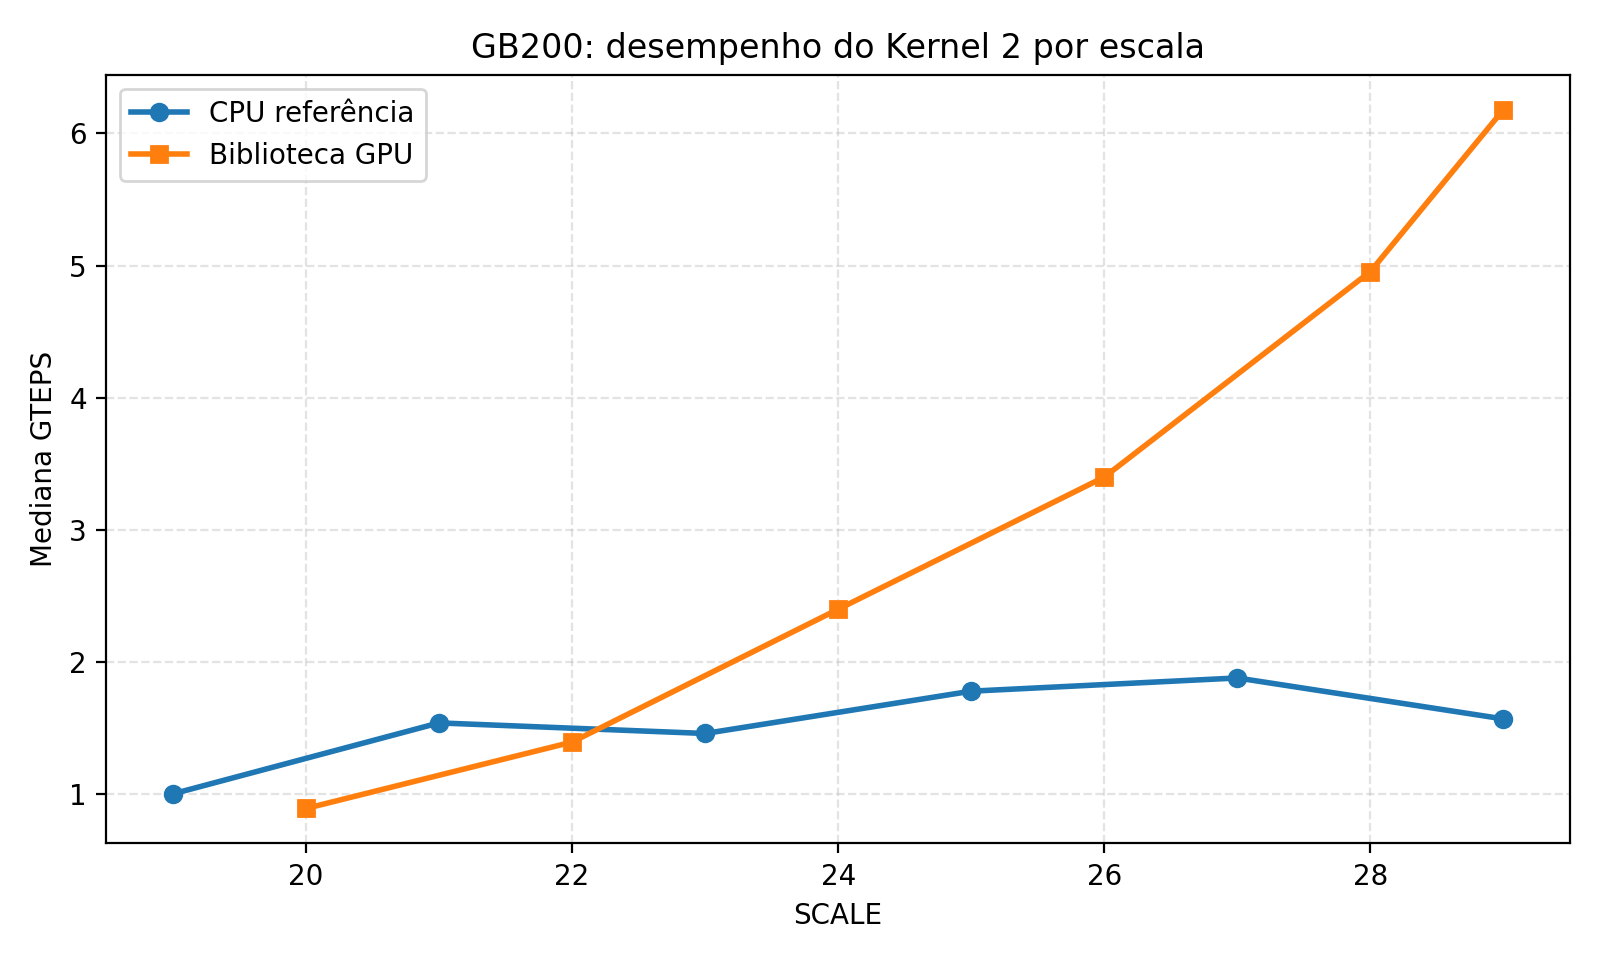
\includegraphics[width=0.9\textwidth]{img/gb200_gteps_por_scale.png}
\caption{Mediana de GTEPS por escala no ambiente GB200.}
\label{fig:gb200-gteps-scale}
\end{figure}

\begin{figure}[H]
\centering
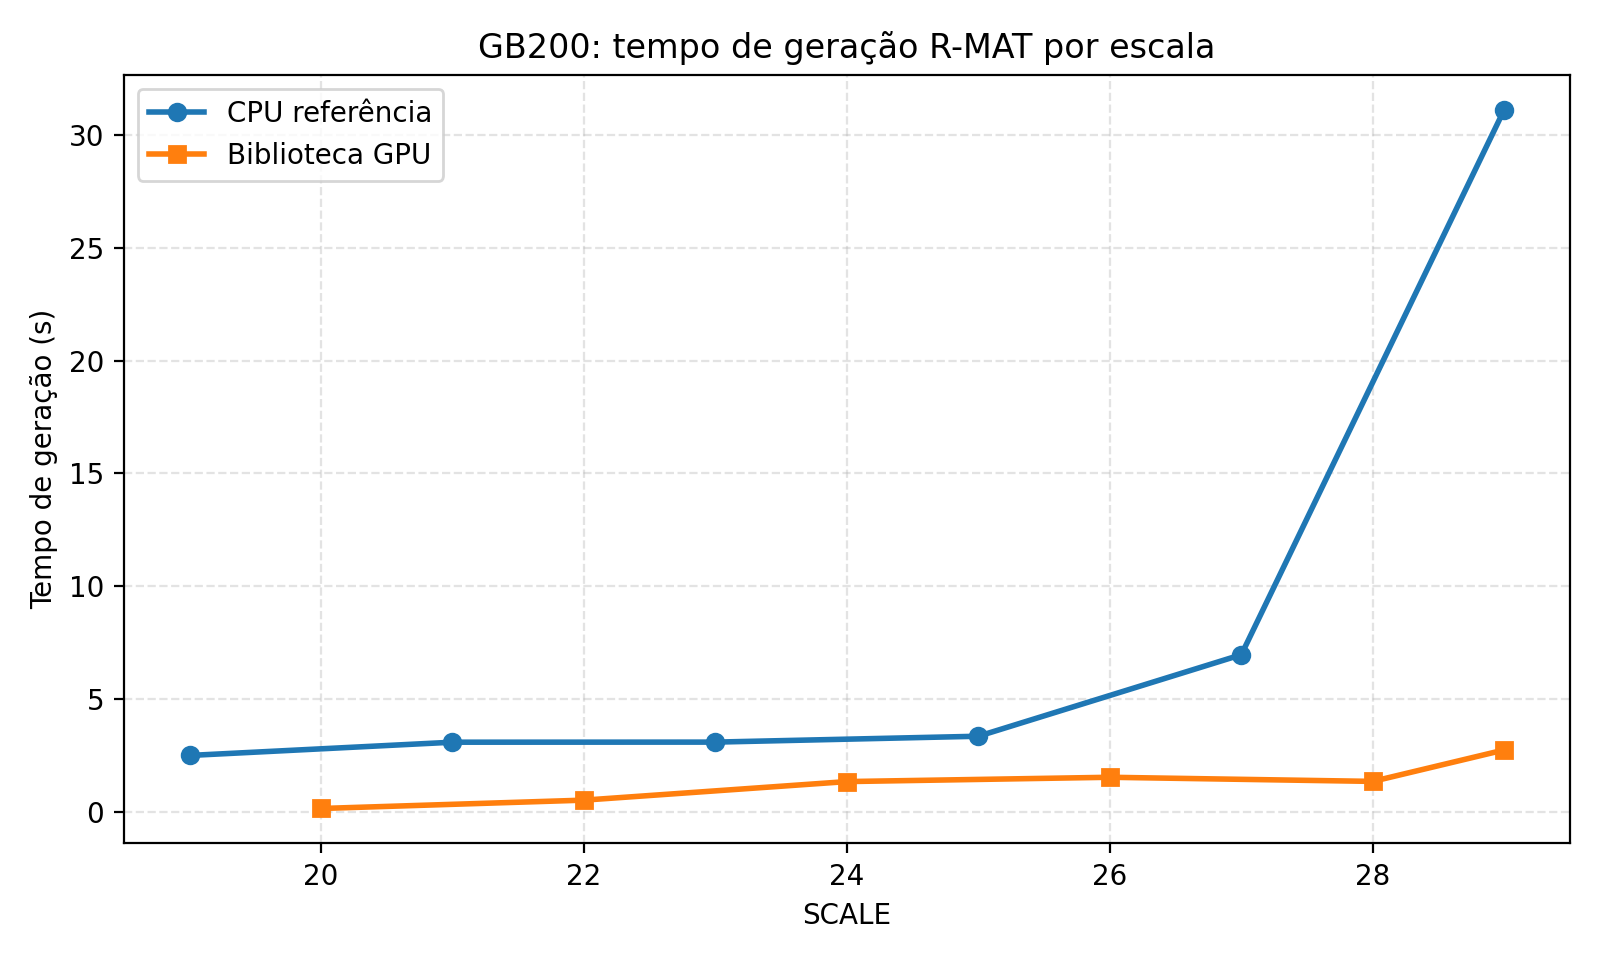
\includegraphics[width=0.9\textwidth]{img/gb200_geracao_por_scale.png}
\caption{Tempo de geração R-MAT por escala no ambiente GB200.}
\label{fig:gb200-geracao-scale}
\end{figure}

No GB200, a biblioteca GPU apresenta crescimento claro de desempenho conforme a
escala aumenta. Como mostra a Figura~\ref{fig:gb200-gteps-scale}, em
\texttt{SCALE=20}, a biblioteca atinge 0,892 GTEPS; em \texttt{SCALE=29}, atinge
6,180 GTEPS. A referência em CPU, por outro lado, permanece entre 1,003 e 1,880
GTEPS nas escalas medidas.

A comparação direta mais clara ocorre em \texttt{SCALE=29}, presente nas duas
implementações. Nessa escala, a biblioteca GPU alcança 6,180 GTEPS, enquanto a
referência em CPU alcança 1,570 GTEPS. O ganho é de aproximadamente $3{,}9$
vezes. O tempo de geração do grafo também é menor na biblioteca, como mostrado na
Figura~\ref{fig:gb200-geracao-scale}: em \texttt{SCALE=29}, a geração leva 2,738
s na biblioteca e 31,13 s na referência em CPU, uma redução de aproximadamente
$11{,}4$ vezes.

Esses resultados mostram que a biblioteca se beneficia mais do ambiente GB200 do
que a versão híbrida se beneficiou do computador pessoal. Isso é esperado, pois o
GB200 oferece mais GPUs e maior capacidade de memória e comunicação. Além disso,
a execução da biblioteca foi projetada para manter a coordenação da BFS dentro da
GPU, o que reduz o custo de controle do host conforme a escala e o número de PEs
aumentam.

\section{Discussão Geral}

Os resultados permitem observar três comportamentos principais. Primeiro, a
geração R-MAT se beneficia fortemente da GPU nas maiores escalas. Isso ocorre
porque a geração é naturalmente paralelizável por aresta e possui menor
dependência de comunicação irregular do que a BFS.

Segundo, a versão CUDA/NVSHMEM híbrida melhora o desempenho do Kernel 2 apenas
nas maiores escalas do computador pessoal. Nas escalas menores, a referência em
CPU é mais rápida, pois o custo fixo da execução em GPU ainda domina. A partir de
\texttt{SCALE=21}, a quantidade de trabalho passa a ser suficiente para que a GPU
supere a CPU.

Terceiro, a biblioteca GPU apresenta ganhos mais expressivos que a versão híbrida.
No computador pessoal, ela supera a versão híbrida nas escalas em comum. No GB200,
ela supera a referência em CPU na escala comum \texttt{SCALE=29}, tanto em TEPS
quanto em tempo de geração do grafo. Isso reforça a principal hipótese do
trabalho: para BFS distribuída em GPU, não basta mover a expansão das fronteiras
para o dispositivo; também é importante reduzir a participação recorrente da CPU
na coordenação entre níveis.

Apesar dos ganhos, os resultados também mostram limitações. A BFS continua sendo
sensível à irregularidade do grafo, à contenção em operações atômicas, à
comunicação remota e ao tamanho das fronteiras. Portanto, os ganhos observados
indicam a viabilidade da abordagem, mas também apontam que a otimização da
comunicação entre PEs permanece essencial para melhorar a escalabilidade da
biblioteca.
